\chapter[Koncepcja rozwiązania własnego][Koncepcja rozwiązania
własnego]{Koncepcja rozwiązania własnego}
Zadaniem projektowym jest wytworzenie rozproszonego systemu plików
przechowującego pliki w~pamięci operacyjnej bądź na~dyskach lokalnych. System
implementowany przez nasz zespół będzie przechowywał pliki na~dyskach lokalnych.

\vspace{5mm}
Usługa podzielona jest na~2 warstwy:
\begin{itemize}
  \item warstwa usług lokalizacyjno-nazewniczych (Master Server),
  \item warstwa właściwego przechowywania (Storage Server).
\end{itemize}

\vspace{5mm}
System opiera się~na~następującej architekturze:
\begin{figure}[H]
\center
\flushleft
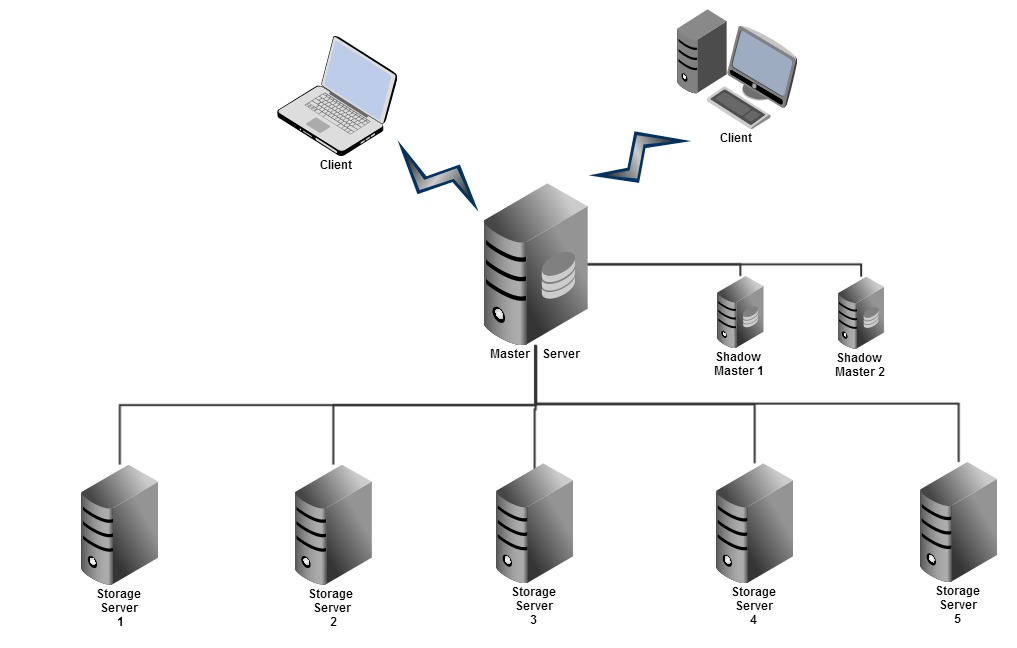
\includegraphics[keepaspectratio=true, scale=0.45]{img/own_conception.png}
\end{figure}

\vspace{5mm}
Master Server odpowiada za~kontakt z~klientem oraz za~przydzielanie plików
do~odpowiednich Storage Serverów. Dodatkowo zarządza bazami danych na~serwerach
lustrzanych (Shadow Server).

\vspace{5mm}
W bazach przechowywane jest drzewo plików załadowanych do systemu, wraz
z~ich~fizycznym miejscem położenia -~identyfikatorami Storage Serverów.

\vspace{5mm}
System zapewnia niezawodność poprzez replikację plików, oraz kopie Master
Servera. Skalowalność jest zapewniona przez~łatwe dołączanie kolejnych Storage
Serverów bez~strat w~wydajności systemu. Rozważano koncepcję odciążenia Master
Servera w~przypadku operacji nie~zmieniających stanu plików (get, status),
które mogły by~być~wykonywane przez~Shadow Servery, jednak dla~zachowania
prostoty zdecydowano by~nie realizować tej~koncepcji.

\vspace{5mm}
System pozwala klientowi ładować pliki do~systemu, pobierać je, usuwać oraz
sprawdzać ich~stan. Podstawowe operacje przedstawiono na~poniższych diagramach:

\begin{figure}[H]
\center
\flushleft
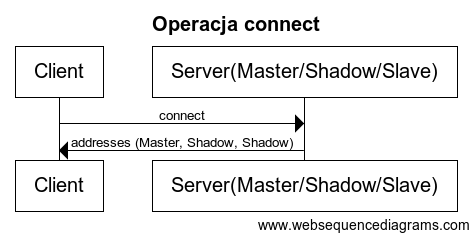
\includegraphics[keepaspectratio=true, scale=0.5]{img/connect_op.png}
\end{figure}

\begin{figure}[H]
\center
\flushleft
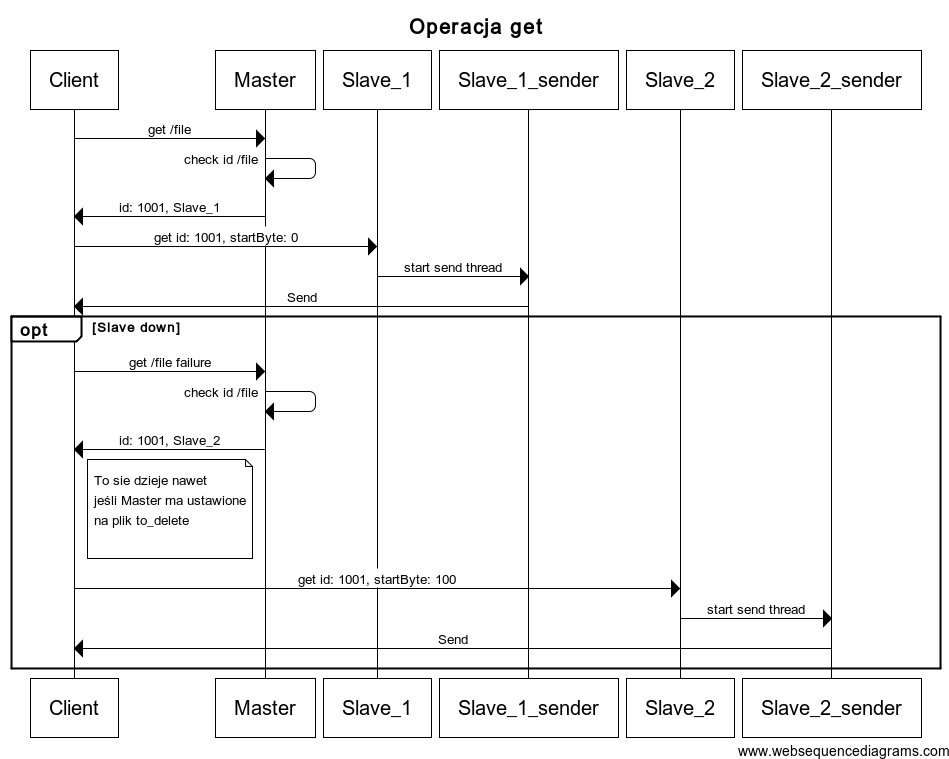
\includegraphics[keepaspectratio=true, scale=0.47]{img/get_op.png}
\end{figure}

\begin{figure}[H]
\center
\flushleft
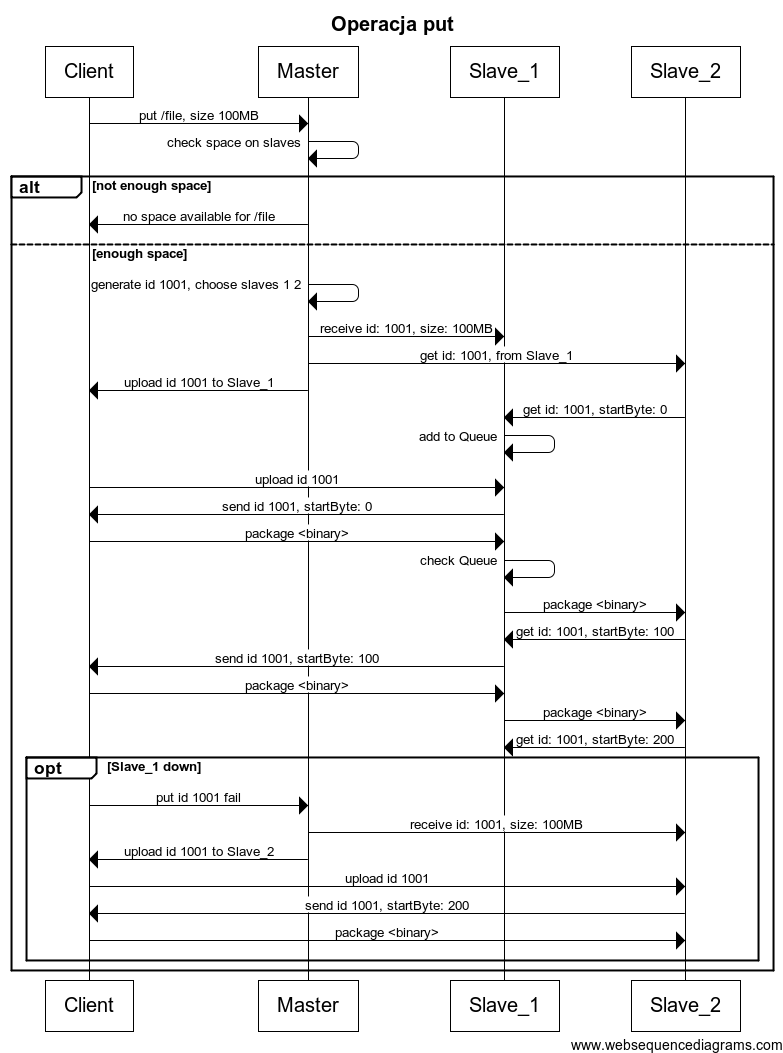
\includegraphics[keepaspectratio=true, scale=0.5]{img/put_op.png}
\end{figure}

\begin{figure}[H]
\center
\flushleft
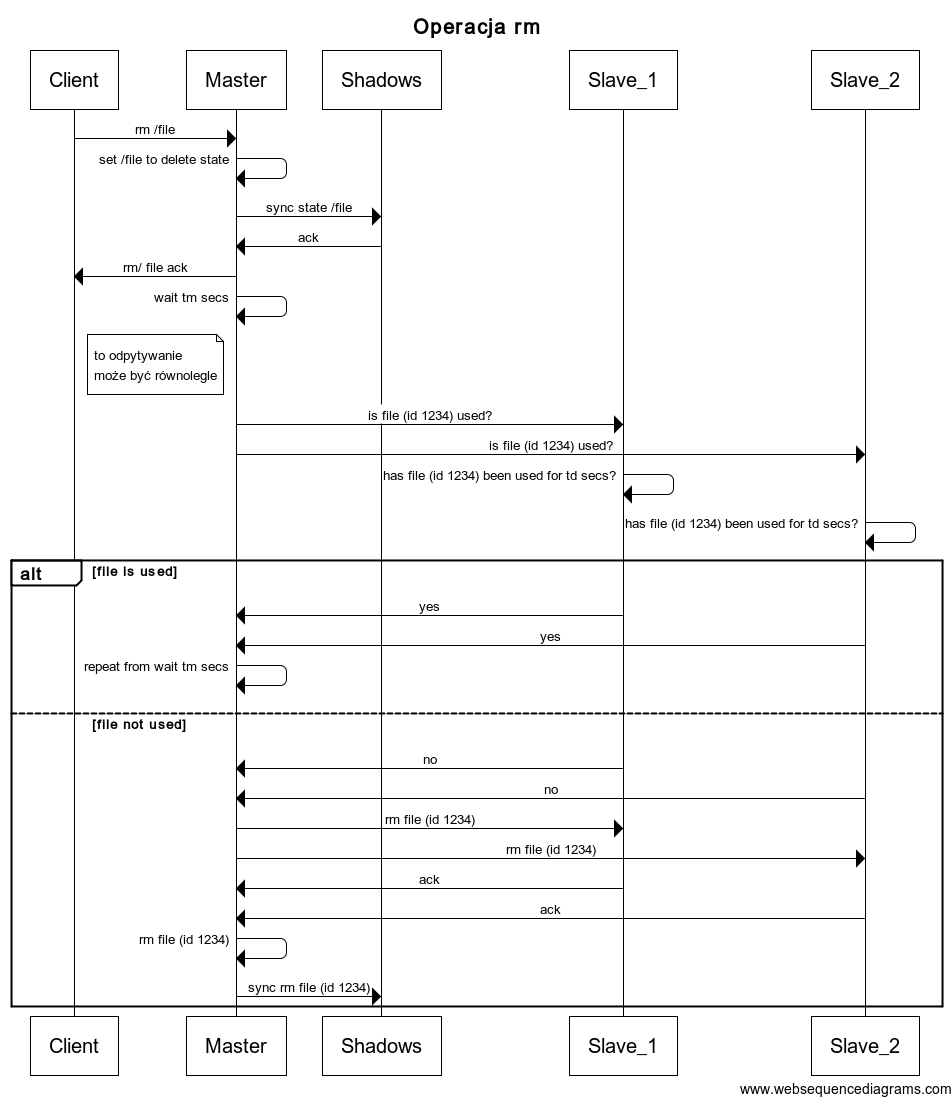
\includegraphics[keepaspectratio=true, scale=0.47]{img/rm_op.png}
\end{figure}

Od strony administratorskiej -~początkowe serwery są~włączane za~pomocą skryptu
uruchamiającego usługę. Operacja przyłączenia nowego serwera, który przez
określony czas nie~odpowiadał, przebiega w~następujący sposób:
\begin{figure}[H]
\center
\flushleft
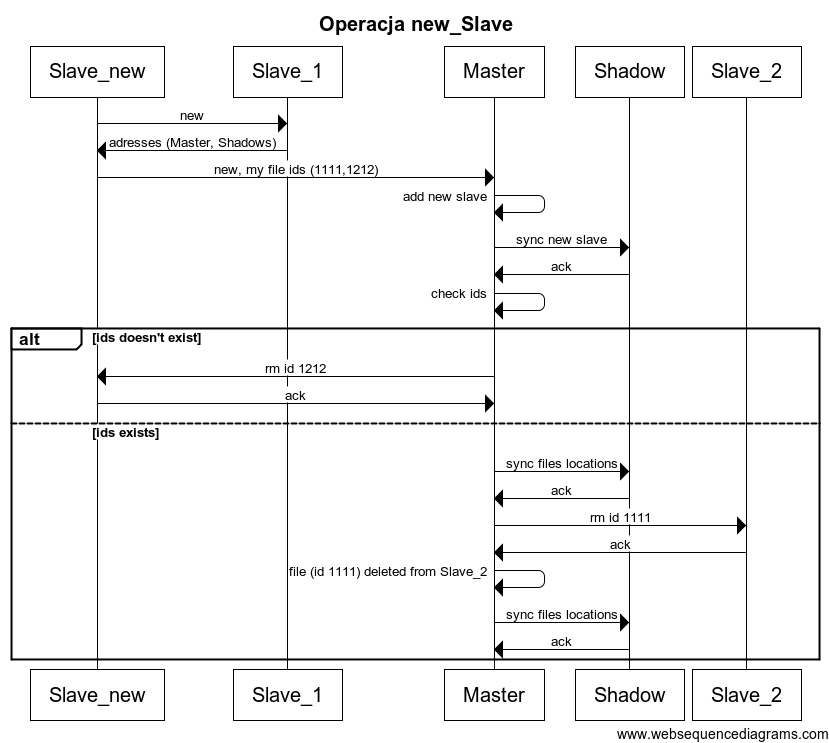
\includegraphics[keepaspectratio=true, scale=0.5]{img/new_slave_op.png}
\end{figure}